\section{Field Study}
\label{sec:field-study}


	The field study took place during the first two weeks of March, from 3/3/2015 to 3/15/2015 in Oettingenstrasse 67, a faculty building of Ludwig-Maximilians-Universit\"at M\"unchen. Data was collected from the displays on 14 consecutive days and 28 semi-structured interviews were carried out on five working days during the same two weeks. A total of 117 interactions were registered with the public display installation and 57 survey responses were recorded.

	The goal of this study was to validate our research questions, and to see how users respond to questionnaires being conducted on displays in the public. We chose to conduct a descriptive study, with a focus on ecological validity, since our research prototype is still in an early development stage. 




\subsection{Research Questions}
	% MOTIVATE: explain why we make this field study, explain what we hope to expect. 
	% > what did we expect from the questionnaires, what from the surveys?

	% Why did we bother to do this study?
	One of the main reasons why we performed this field study, was to get a better understanding of our assumptions and to see how users react to questionnaires on displays in public. Besides, it was of importance to conduct a study ``in the wild'', because there often is a discrepancy between lab studies and field studies. This phenomena has been discussed by Ojala and Kostakos in 2011: ``The first important conclusion we have arrived at is that there exists a huge difference between results obtained in a lab and in the wild using the exact same configuration''\cite{Ojala2011}.

	% What do we assume  /  What do we want to know
	An assumption we made for the development of our first research prototype of the PDSurvey platform was that we can simplify the conduction and deployment of surveys to large public display networks. Since this is a rather large claim, we broke down this hypothesis to more fine-grained statements. 
	% NOT / chapter crossed out: 
			%The claim, whether the PDSurvey platform facilitates the conduction of large-scale surveys in public, will be evaluated in the following chapter (see chapter \ref{sec:expert-interview}). 

	We already had an application running on a public display in a faculty building which attracted lots of regular and new users. Our interest was how we could best integrate questionnaires on and after the application itself (a balloon shooter game, see section \ref{sec:field-study:apparatus}).

	The following research questions are the basis for the field study:

	\begin{enumerate}
		\item Which channels are best suited for completing surveys in public?
		\item Why did the users approach the display? What motivates them to fill in surveys in public? 
		\item How did the user notice and perceive the survey on the display?
		\item Which question types are best suited for questionnaires carried out in public? 
	\end{enumerate}

		% Optional questions >>> MAYBE TAKE ALL OF THESE AND ADD THEM TO FUTURE WORK
		These four research questions were represented in the PDSurvey and semi-structured interviews. Due to the time restriction of this Master thesis could be assessed which came up during the literature review phase. Questions which would go beyond the scope of this thesis, and might serve as follow-up questions for further research, are gathered here:

		\begin{itemize}
		\item In which situations is the user most willing to answer surveys on public displays? What influence does the context and surrounding environment have on the survey responses?
		\item How many questions are acceptable and tolerated? Does this variable differ between the feedback channels, location of the display setup, and its surrounding environment? Which other factors play a role here?
		\item What is the ideal placement for surveys to pop up on a public display? Where should an overlay be positioned, when embedding it into a foreign application? How large/small, how obtrusive should it be?
		% \item According to Joerg Mueller: the best position on large public displays is directly in the center (not at the bottom, not at the top, close to the center). The larger the screen is, the more relevant a centric positioning will get.
		\item Getting a better understanding of the influence of the environment, e.g. how personal questions can get in public, and how much privacy the display should offer (the smaller the display, the more private the context seems).
		\item How can we best break down a standardized survey with 10+ questions across multiple users, each getting their own subset of questions?
		\end{itemize}

	In addition to these questions we were also interested in user stories, in the feedback real-world users gave us in regards to answering surveys on screens in the public. For this reason we also conducted semi-structured interviews in parallel to the quantitative evaluation of the PDSurvey platform. In order to get as authentic and personal feedback as possible, we stuck only roughly to the designated questions of the semi-structured interview (see Appendix \ref{appendix:interviews}).




\subsection{Study Setup}
	% give the reader enough information to replicate the experiment

	A descriptive research type was as the study type, aiming to describe and observe how users react to the new display setup. One single prototype is deployed, without varying any variables. The goal was to get first feedback on how people perceive filling in questionnaires in public, before getting into more fine-grained research (see Future Work, chapter \ref{sec:future-work}). 
	Both quantitative and qualitative data was gathered as part of the field study. Quantitative data was obtained through the PDSurvey system and qualitative data was collected through semi-structured interviews.



	\subsubsection{Design}
	\label{sec:field-study:design}


	% Goal: Which Feedback Channel
	Our primary goal was to find out which channel users preferred to respond to surveys in public. Each user had the choice to respond to the questionnaire on a TV display, on a tablet to the right of the TV screen, via their own smartphone or via email. We displayed the same five questions on all four feedback channels (see Table \ref{table:5-questions-asked}). We chose to limit the number of questions asked via all four channels to 5, to avoid a low participation and response rate. 

	% Questions
	\begin{tabular}{lc}
\toprule
\textbf{Wording}                                                     & \textbf{Question Type} \\ \midrule
1. How often have you used this display before?                         & Numeric                \\
2. How likely is it that you will use this display in the future again? & 5-point Likert scale   \\
3. Which devices do you possess or use regularly?                       & Multiple choice, 5 options                        \\
4. In which area do you study / work?                                   & Text field             \\
5. What was your motivation for approaching and using this display?     & Text field            \\
\bottomrule
\end{tabular}


	% I: QUESTIONNAIRE

	% Question Types
	In order to also get first insights into how well certain question types are suited for surveys in public, where a short completion time is crucial, we varied between the following question types and kept them in the same order: numeric questions, Likert scale, multiple choice (based on check boxes) and two text fields for responses of undefined length. 

	% Intrinsic motivation
	To increase the motivation for participation, additional intrinsic motivation was given to increase the response and acceptance rate of the public surveys, as proven by Richard Ryan in his self-determination theory\footnote{http://www.selfdeterminationtheory.org/} \cite{ryan2000self}. We stated that the questionnaire consists of five questions, that it will only take one minute to complete and the results are for a Master's thesis at the university. This information was displayed as a splash screen on the tablet (see Figure \ref{fig:5-pdclient-intro}).

	\begin{figure}
	    \begin{center}
	        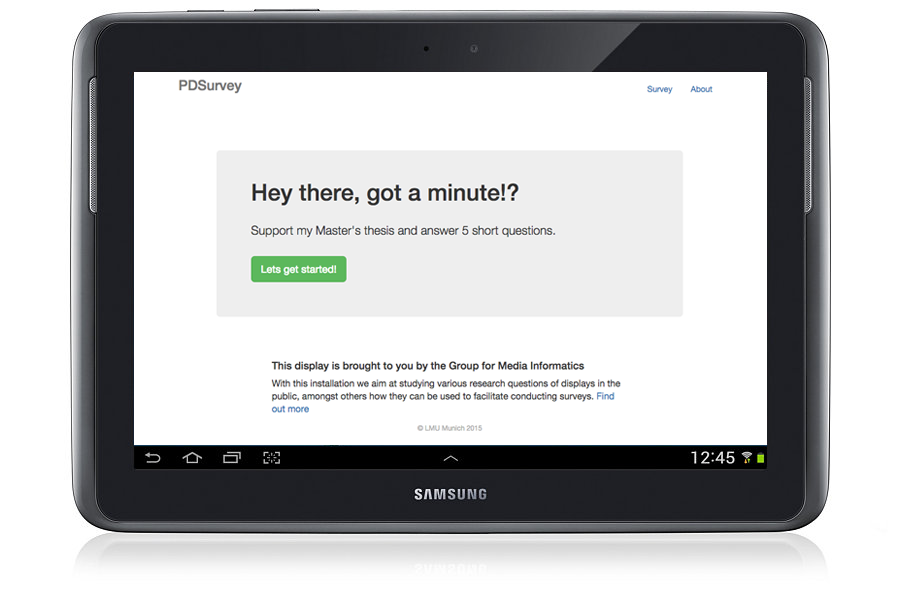
\includegraphics[width=.7\columnwidth]{img/5_field-study/pdclient-startscreen.png}
	    \end{center}
	 \caption{PDClient: Motivating users to participate in a short questionnaire}
	 \label{fig:5-pdclient-intro}
	\end{figure}

	% Study setup: pure observation (no indep. variables / conditions)
	Since we conducted a descriptive study, we only observed how users used our study setup. The parameter of interest was the feedback channel chosen to respond to the survey. Due to the fact that we didn't have any conditions, no independent variables are present.

	% II: SEMI-STRUCTURED INTERVIEW

	To find out more about the users motive for approaching the display setup, we also carried out semi-structured interviews in parallel to the field study of the PDSurvey platform. The goal of the interviews was to get qualitative feedback from all age groups and backgrounds. Getting a better understanding of how people respond to questionnaires in public, helps us develop the PDSurvey platform more target-orientated.




	\subsubsection{Participants} % provide the necessary information about the people who took part in your experiment

		In total 54 questionnaires were submitted and 28 semi-structured interviews were conducted during the two week study period. As for the study size, we took the findings from Alt et al.\cite{Alt2012HowToEvaluate} as a rough guide, according to which most field studys have an average of 26.9 interviews and 38.4 questionnaire responses.

		Questionnaires were completed mainly by students, but with various backgrounds. Since our research focus was to find which feedback channel is best suited for conducting automated questionnaires in public, we only included one question in the quantitative PDSurvey questionnaire to collect demographic data. 

		Based on the fourth question (``In which area do you study / work?'') we can draw a conclusion about the study field of the survey participants. Out of the 54 questionnaire responses 42 submissions could be assigned to a study field. The remaining 12 submissions consisted of responses such as \textit{bavaria, bib, home, munich, muc} or were left empty. The study fields most frequently represented were Computer Science (23,8\%), followed by Political Science (14.3\%), Japanese Studies (11.9\%), and Anthropology (11.9\%). Other study fields mentioned were Cultural Science, Business, Physics, Sociology, Ethnology, Communication Science, Sports, and Science \& Technology. 

		For the semi-structured interview we collected more detailed information about demographics of the participants. Out of the 28 participants,
		20 were male and 18 were female. The age of all people interviewed ranged between 20 and 69, with an average age of 31,5 years.	Due to the wide variety of faculties and a library being located in the same building, various technical backgrounds were present. What they all had in common was their affiliation to LMU Munich, either because of being a student themselves, working at the university or being otherwise related to the university. In total 23 students, three employees, and two retirees were interviewed. The study fields which were most frequently represented are Computer Science (16.7\%), Japanese Studies (16.7\%), Ethnology (12.5\%), and Political Science (12.5\%). Other areas mentioned were Sociology, Communication Science, Law, Physics and Engineering. The full list of demographics, including exact ratios, can be seen in Table \ref{table:demographics}.


		\begin{table}[h]

			\begin{tabular}{lllll}
\toprule
   & \textbf{Participants Of Survey} &  &   & \textbf{People Interviewed}                        \\
   \midrule
10 & Informatics                            &  & 4 & Informatics                                        \\
6  & Political Science                      &  & 4 & Japanology                                         \\
5  & Japanese Studies                       &  & 3 & Ethnology                                          \\
5  & Anthropology                           &  & 3 & Political Science                                  \\
4  & Cultural Science                       &  & 3 & \textit{employees} (PhD, public officer, SysAdmin) \\
4  & Business                               &  & 2 & \textit{in pension}                                \\
2  & Physics                                &  & 1 & Communication Science                              \\
2  & Sociology                              &  & 1 & Sociology                                          \\
1  & Ethnology                              &  & 1 & Law                                                \\
1  & Communication Science                  &  & 1 & Physics                                            \\
1  & Sports                                 &  & 1 & Engineering                                        \\
1  & Science and Technology                 &  &   &               \\
\bottomrule
\end{tabular}

			\caption[Demographics of Field Study]{Demography for the survey data (left) and the semi-structured interview (right).}
			\label{table:demographics}
		\end{table}


		% HOW WE OBTAINED THE PARTICIPANTS
		The selection of the participants for the completion of the surveys was not influenced by us. All survey responses were made in their own interest, no reward was given for participating in this ``in the wild''-study.
		The selection of the participants for the semi-structured interview was influenced by how users reacted to the display setup. Our primary goal was to observe and interview active users of the public display setup, in order to get a better understanding of how they perceived the setup and to get insights into which feedback channel they chose why. In order to also understand why people did not approach, or if they have any concerns, people passing by were also interviewed. 

		% CONDITIONS \item how many took part in which condition
		
		Before starting the semi-structured interviews, all people participating were asked whether they have previously noticed the display setup and/or the option to fill in a survey. 

		This allowed us to differentiate three groups: participants who approached the display by themselves (and were observed doing so), people passing by the display (noticing the display, however not approaching it) and the last group of people simply passing by (not having noticed the display). The distribution between the groups was as follows: 11 active participants, 17 passerby (14 noticed the displays before, 3 haven't). 

		Out of all people passing by no one has noticed the option to fill in a survey. Out of the active participants, 4 out of 11 have noticed the option to respond to a survey on different channels.

		To increase the amount of feedback, we approached people from all three groups. The number of survey responses was not artificially increased by asking passersby was.


		% MENTION RELEVANCE OF FIELDS (MAYBE)
		\textbf{> TODO: think about which information is RELEVANT and which is not! for me the devices they possess might be of relevance. people not possessing a smartphone or tablet, might be less willing to use these devices.} 
		

		% have noticed displays?
		... and 25 out of 28 noticed the public display setup before. For three people interviewed it was the first time that they have noticed the displays.




	\subsubsection{Apparatus}
	\label{sec:field-study:apparatus}
		% give details of any equipment used, including thinkgs like questionnaires and other tests

		The permanent setup consisted of a XXX-inch TV screen, connected to a laptop running Windows 7, and a Samsung Galaxy Tab 10.1 tablet positioned to the right of the TV screen on a console. Our object of investigation was the TV screen with touch support, running an interactive game called \textit{Balloon Shooter}, developed by Jiamin Shi. After users completed the game, they were asked via a notice to fill in a questionnaire on one of the four provided feedback channels (see Figure \ref{fig:5-feedback-options}). The courtesy for the Balloon Shooter game and the survey implementation on the TV screen goes to Jiamin Shi.

		\begin{figure}
		    \begin{center}
   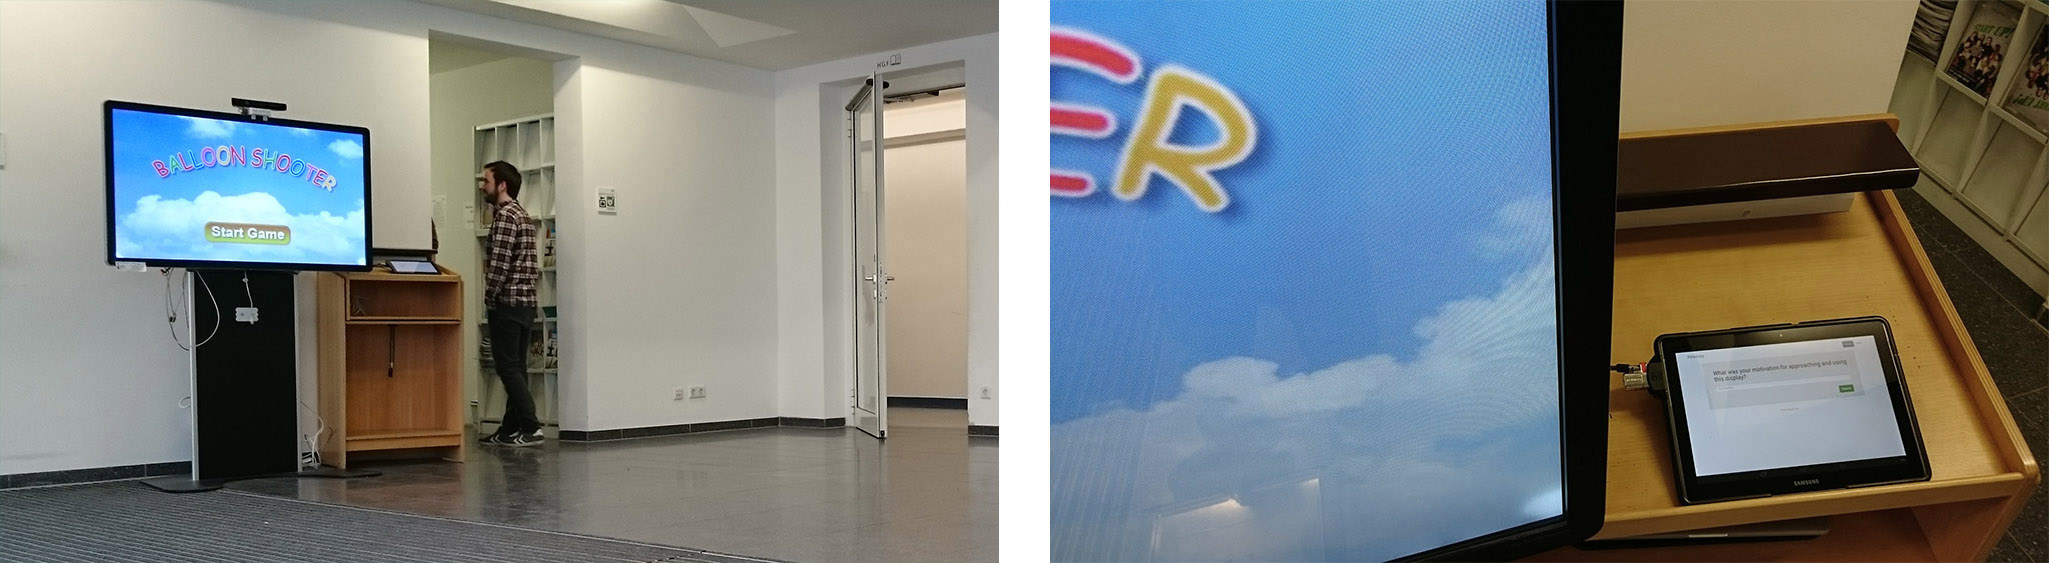
\includegraphics[width=\columnwidth]{img/5_field-study/study-setup.jpg}
		    \end{center}
		 \caption{Overview of the study setup in the entrance hall of the faculty building.}
		 \label{fig:5-study-setup}
		\end{figure}

		Each user had the opportunity to respond to the questionnaire either directly on TV screen (1), on a tablet to the right of the big TV (2), via their own smartphone (3) or via email (4). The first option was embedded natively into the Balloon Shooter game, offering a consistent UI and the most direct feedback channel. Choosing the tablet as an option, the users were prompted to move to the right and to answer five questions on the tablet. The Samsung Galaxy Tab 10.1 was displaying the responsive frontend of PDClient, being enclosed in an Android Kiosk App, namely KioWare Lite\footnote{http://www.kioware.com/android.aspx}. Choosing the third option prompted the user to either scan a QR code with their smartphone or to open a URL in their mobile browser. The last option consisted of an input field embedded into the Balloon Shooter game on the TV screen, asking the user to enter their email address. The address was logged to a txt-file, which was scanned every 5 minutes by a Windows task scheduler. An email reminder was sent to the user with the request to complete the survey. For sending the email from the TV screen a Python script was written to send the email via the universities SMTP server\footnote{https://github.com/lukasziegler/python-send-mail}. Screenshots of all four options can be found in the Appendix on page \pageref{appendix:screenshots-balloon-shooter}.

		For the permanent setup the following data was logged on all four feedback channels: The timestamp of the users choice, which feedback channel the user chose to respond to the survey, and whether they skipped the call to participate in the survey or if they stopped playing the game (determined via timeout). 

		% maybe also show a flow of actions, but not sure if this is needed, when the user can also simply read the previous paragraph.


		% II) SEMI STRUCTURED INTERVIEW
		For conducting the semi-structured interviews two questionnaires (one for participants, one for passerby), a voice-recorder (smartphone) were used in addition to the permanent setup.

		For the evaluation in the field study itself a self-made questionnaire was used, since the focus was on finding which channels and question types are best suited in general for being used on public display. This was the reason why we did not use any of the standardized questionnaires mentioned in section \ref{sec:questionnaires}. Screenshots of the questionnaire run on the PDClient can be found on the enclosed CD.




		% III) BALLOON SHOOTER GAME

		% More information regarding the Balloon Shooter game can be found here XXXXX. 

		The main application installed on the public display was a game called \textit{Balloon Shooter} developed and run by Jiamin Shi, a PhD student at the Group for Media Informatics at LMU Munich. It was first installed on January 7th 2015 and has been running in different versions since then. Public audience was already used to it for roughly two months and adapted to it well.

		% + give more information about the balloon shooter game.
		% + ask Jiamin, whether and which screenshots of the game I am allowed to post?




	\subsubsection{Location}

	All parts of the field study were carried out in Oettingenstrasse 67, the faculty building for Computer Science. In the same building there are also research institutes for Ethnology, Political Science, Japanese Studies, and Physics. The study was carried out in the entrance hall of the university building. Figure \ref{fig:5-entrance-hall} gives an overview of the entrance hall and of the paths most people take while crossing the room. The excerpt is based on the universities floor plan\footnote{\url{http://www.uni-muenchen.de/funktionen/gebaeudeplaene/7070_d_00.pdf} (last visited on March 22, 2015)} and was inspired by Sandra Zollner \cite{zollner2014thesis}. There she also published that at the time of her study ``approximately 59\% of all passers-by used path 1'', to get something from the lockers or to leave through the door to the library. 28\% of the people were taking path 2 and 13\% were taking path 3.

	\begin{figure}
	    \begin{center}
	     \fbox{		        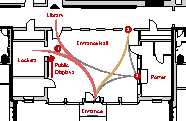
\includegraphics[width=.7\columnwidth]{img/5_field-study/entrance-hall.pdf}
	     }
	    \end{center}
	 \caption[Floor Map of Entrance Hall]{Floor map of the entrance hall, where the field study was carried out. User paths, and the surrounding environment including facilities such as the library can be seen.}
	 \label{fig:5-entrance-hall}
	\end{figure}

	In our field study it was also evident that the majority of the visitors took path 1 were usually fairly target-orientated or in a hurry. Otherwise, on days with bad weather people had their break in the entrance hall or waited for someone. On days with good weather people usually took their breaks outside and only passed through the entrance hall, coming from the library, picking up something from the locker room and going outside.


	\subsubsection{Procedure}
		% tell the reader how the study was carried out in practice

		All participants of the semi-structured interview were asked a similar set of questions (see Appendix \ref{appendix:interviews}). Based on the group they belonged to, either questionnaire 1 (for participants of the display setup) or questionnaire 2 (for passersby) was chosen. In order to speed up the interviewing process and to get away from a plain question-response schema, the questions on the printed out questionnaire only survey as a rough guideline. 

		% Instructions given
		For people having trouble understanding the concept of the public display installation, the situation was described as follows. ``Imagine you are in a shopping mall or at an airport using one of those large displays to find some information. After having found what you were looking for, you get asked to answer a short questionnaire. How would you react to it?'' A full transcription of all questions and responses can also be found on the enclosed CD. 

	% Adjustments on the day prior to the evaluation
		% The day prior to the launch of the actual field study was used for assembly and for last adjustments, like change of font size, adjustment to the position of certain UI elements, and for collecting implicit feedback from users observing but not approaching the display. From observing it could be seen that a more effective call-to-action was needed. Many people looked at the display, noticed that something has changed with the setup, but no one started interacting with the new setup or was willing to complete the questionnaire. Therefore a more catchy start screen was introduced for the tablet (see \ref{fig:5-pdclient-intro}) and the option panel of the TV screen was also modified \ref{screenshot:options}. This observation is very much in line with the self-determination theory by Richard Ryan and Edward Deci \cite{ryan2000self}.


		\begin{figure}
		    \begin{center}
				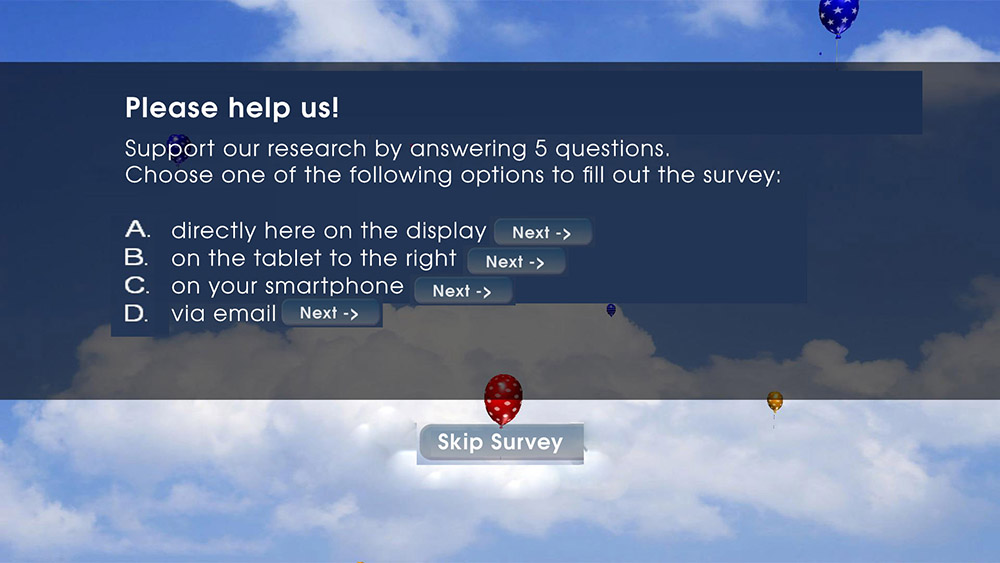
\includegraphics[width=.8\columnwidth]{img/screenshots/options-overview.jpg}
		    \end{center}
		 \caption{Options panel to choose a feedback channel}
		 \label{fig:5-feedback-options}
		\end{figure}


		The participants for the PDSurvey questionnaire were not additionally motivated. All they saw was the options panel after completing the Balloon Shooter game (see Figure \ref{fig:5-feedback-options}) or the welcome screen of the tablet (see Figure \ref{fig:5-pdclient-intro}) while passing through the entrance hall. A complete copy of what the users were able to interact with, can be seen on the attached CD (see Appendix \ref{appendix:cd-contents}).


		% REMINDER: only give RELEVANT information to the reader!
		% > only provide details if they are needed for replication
		% > or if they are relevant to the outcome of the experiment




\subsection{Results}

%%% QUANTITATIVE DATA %%% = pure facts
	% just tell the reader what you found

% I) Descriptive Statistics
% - provide summaries of group performance
% - present: average, mean, mode
% - describes: standard deviation, range (how it is spread)
% - describes: frequency of data (if relevant)

% presentation of data
% - don't present data multiple times
% - either use a TABLE or a GRAPH
% always explain to the reader in words what the results show
% - tables / graphs should be self explanatory
% - the text should be comprehensible without taking a look at the figures


	We received a total of 57 filled in surveys, submitted via all four of the provided feedback channels, and carried out 28 semi-structured interviews. 
	No treatments were applied to the dataset, descriptive statistics will follow bellow. The presentation of the evaluation is divided into three parts. First we will have a look at which feedback channel is most popular, followed by the quantitative results of the PDSurvey questionnaire, and rounded off with the results from the semi-structured interview. 

	%% OLD VERSION
	% Section \ref{5:results:demographics} describes the demography and background of the participants, while section \ref{5:results:feedback-channel} containing an evaluation of which feedback channel was preferred in the survey responses and interviews, combined with reasons stated from the semi-structured interviews. In section \ref{} 


	\subsubsection{Feedback Channels}
	\label{5:results:feedback-channels}
	\label{5:results:feedback-channel}

	\textbf{NOT SURE HOW TO BEST POSITION THIS PART}

	The majority of the surveys were submitted on the tablet (87.72\%). Four responses were recorded directly on the TV (7.02\%), two via smartphone (3.51\%), and one via email (1.75\%). Since this listing only contains the number of responses, it should not be taken as a base for the comparison of the feedback channels' popularity. %% interpretation !! %% 
	Due to the tablets sole purpose to be used to fill in surveys in our setup, and the additional intrinsic motivation given on this channel (see section \ref{sec:field-study:design}), this ratio has to be treated with caution. For a comparison of the \textbf{feedback channels} the log data from the option panel and the responses from the semi-structured interviews are better suited (see Table \ref{table:5-feedback-channel}).


	% PREFERRED CHANNEL
	After having completed one session of the game, users had the option to choose a feedback channel. Based on this log data of the TV screen a better comparison of the feedback channels can be made, since all direct responses made on the tablet are excluded from this summary. The most popular feedback channel was the tablet (46.15\%), followed by the TV screen (30.77\%), smartphone (15.38\%), and email (7.69\%).
	% based on >Interviews
	In order to have another source of input, the same question was asked at the end of every semi-structured interview. Based on this quantitative data from the interviews the response via tablet (42.86\%) was most popular again, followed by the TV screen (32.14\%). Interestingly, for the interview data the option to respond via email (17.86\%) is more popular than smartphone (7.14\%). 
		
	\begin{table}[h]
\center
\begin{tabular}{lllll}
\multicolumn{2}{l}{\textbf{From Survey Data}} &  & \multicolumn{2}{l}{\textbf{From Interviews}} \\
30.8\%                   & \multicolumn{3}{l}{on public display}      & 32.1\%                  \\
46.1\%                   & \multicolumn{3}{l}{on tablet}              & 42.9\%                  \\
15.4\%                   & \multicolumn{3}{l}{on smartphone}          & 7.1\%                   \\
7.7\%                    & \multicolumn{3}{l}{at home / via email}    & 17.9\%                 
\end{tabular}
\caption[Feedback Channel]{Preferred feedback channel for answering surveys.}
\label{table:5-feedback-channel}
\end{table}






	\subsubsection{Survey Responses}
	\label{5:results:survey}
	%% Evaluation of all five questions



	% DONT USE SUB HEADINGS, THE FLOW SHOULD BE CLEAR WITHOUT 

	\paragraph{How often have you used this display before?}
	% 1) How OFTEN have the users USED this display BEFORE?
	In our questionnaire executed on the public displays we asked five questions. Out of the 57 responses people have on average used the display 6.9 times before. For 25 people (43.9\%) of the users it was the first time using the display setup, 11 people (19.3\%) have used it once before, 18 people (31.6\%) between two and ten times, and the remaining 3 people (5.3\%) more than ten times.

	\paragraph{How likely is it that you will use this display in the future again?}
	% 2) How LIKELY is it that you will USE THIS DEVICE AGAIN?
	For the second question, based on a 5-point Likert scale, the response was fairly uniformly distributed (average=3.04, SD=1.46). The whole scale from 1 (not likely at all) to 5 (very likely) was represented. No clear trend could be seen. When only considering the responses collected from the large TV screen, a better perception can be noticed. There the responses to this question had an average of 4.5 (SD=0.866), showing a trend towards a positive perception of the large display setup. However, due to the low number of responses for the TV display, this conclusion can not be regraded as significant. 

	\paragraph{Which devices do you possess or use regularly?}
	% 3) DEVICES the users possess
	Taking a look at the devices users possess might give us first insights into why users chose which feedback channel. Overall, the majority of the people participating in the survey already owned a smartphone (79.3\%). The second most popular response was laptop (73.6\%), followed by tablet (41.5\%), and desktop computer (26.4\%). Still, 18.9\% of the users indicated that they possess a feature phone and use it regularly. On average each participant possessed 2.4 devices. 
	When looking at which combinations of devices were most frequent, twelve people responded that they own a smartphone + tablet + laptop. Twelve other people indicated that they possess a smartphone + laptop, and six people own a smartphone + laptop + desktop.

	% 4) Study area >> demographics
	\paragraph{In which area do you study / work?}
	The fourth question was used to get a little insight into the background of the survey users. Only the occupation of each participant can be derived from the questionnaire. As far as was indicated all people responding to the questionnaire installed on the public display setup were students. The majority of people interacting with the TV screen study Coputer Science (23.8\%), followed by Political Science (14.3\%), Japanese Studies (11.9\%), Anthropology (11.9\%), Cultural Science (9.5\%), and Business (9.5\%). Table \ref{table:demographics} shows a full list of which study field or work field the participants specified.

	% 5) REASONS FOR APPROACHING
	\paragraph{What was your motivation for approaching and using this display?}
	The main reasons why people have approached the display were ``curiosity'' (12x), ``fun'' (10x), ``boredom'' (8x), ``interest'' (2x), and ``during breaks'' (2x). Other reasons mentioned were ``it is there, so why not?'', ``it is there and colourful'', or ``I've never seen it before in this spot, wanted to know what it is about''.




%% INTERVIEW DATA >> QUALITATIVE RESULTS > a combination of facts + evaluation

	\subsubsection{Interview Responses}

	As mentioned earlier, we also conducted semi-structured interviews. The evaluation of the semi-structured interviews was based on Grounded Theory, for a systematic evaluation of the interview transcripts. A total of 28 semi-structured interviews were conducted, of which 72.4\% of the participants were male and 28.6\% were female. The average age was 31.5 years, with an age distribution ranging from 20 years up to 69 years (median=25.5, SD=13.2). Eleven of the 28 interviews were conducted with actual participants of the public display study setup (39.3\%), the remaining 17 interviews (60.7\%) consisted of people passing by the display. 

	To avoid any interferences between the two groups, each passerby was asked before starting the interview whether he has noticed the public display installation, and whether he has already interacted with the installation. Out of all passerby no one has previously been interacting with the game or survey platform. 82.4\% (14 of 17) of the passerby have already noticed the public display installation before, however, none of the passerby has previously participated in the game. The remaining 17.6\% have neither approached the display nor noticed it previous to the interview. 

	Looking at the scientific background of all 28 participants, 79.2\% are students, the remaining 20.8\% either already worked full-time or were in pension. The majority of students studied Computer Science (16.7\%), Japanese Studies (16.7\%), Ethnology (12.5\%) or Political Science (12.5\%).

	From what has been mentioned, the main reason for approaching the public displays was in 6 out of 8 cases ``curiosity'' (6x). Two other reasons were ``for fun'' (1x) and ``waiting for someone'' (1x). Reasons for not approaching the display were ``no time'' (2x) and ``it is in the entry zone of the university, it feels strange when one plays with it'' (1x).

	% OPEN CODING PHASE
	From the open coding phase the following patterns can be seen: 

		\textbf{ASK JULIE!}

		- reason for approaching: see above
		- number of questions found acceptable: 5 - 10
		- reasons for choice of feedback channel: 
		- requirements for a survey, to attract users: 

		- most interesting feedback: reason PRO / CON using a certain channel

	% Reasons mentioned for choice of feedback channel
	The semi-structured interview was most useful to get a better insight into why certain users chose which feedback channel. Reasons mentioned influencing their choice were ``''
	
	see Table \ref{table:interview-coding}.

	  % 1) TV SCREEN
  \begin{table}[h]
    \small
    \center

    \begin{tabular}{p{7cm}p{7cm}}
    \toprule
    \textbf{Pro ``TV Screen''}  &  \textbf{Contra ``TV Screen''} \\ \midrule

    4x Most direct, immediate feedback  &  4x Display is too large  \\
    2x I am already standing here (2x)  &  3x Feels too public  \\
    1x Seems easiest  &  2x Everyone could watch me  \\
    1x Requires less personal information  &  1x That is mean, when the screen is so large  \\
    1x All on one device  &  1x The keyboard on the display would have been too large and confusing  \\
    1x I can use it without putting my glasses on  &  1x Display is uncomfortable for reading long questions  \\
    1x Seems to be the fastest option  &  1x Don't feel comfortable standing in focus in such a large room  \\

      &  1x The system is too innovative, that is why I wouldn't trust it yet \\
      &  1x Because of social desirability influencing my responses  \\

    \bottomrule
    \end{tabular}

    \caption[Feedback Channel - TV Screen]{Reasons mentioned for/against using the \textit{TV screen} as a feedback channel.}
    \label{table:feedback-channel-TV-screen}
  \end{table}

 

  % 2) TABLET

  \begin{table}[h]
    \small
    \center

    \begin{tabular}{p{7cm}p{7cm}}
    \toprule
    \textbf{Pro ``Tablet''}  &  \textbf{Contra ``Tablet''} \\ \midrule
    5x The display is smaller and better laid out)  &  2x Redundancy (``why do I need a tablet when I can respond on the TV screen?'') \\
    2x Better sensitivity / user experience  &  1x Personal aversion (he had bad experiences with tablets) \\
    2x It feels more private  &   \\
    1x Because it is its sole purpose  &   \\
    1x You are not in the way of others  &   \\
    1x I am more used to it  &   \\
    1x Most interactive option  &   \\
    1x Less people watching  &   \\
    1x Because I expect a better input  &   \\
    1x Requires less personal information  &   \\
    1x More comfortable standing here  &   \\
    \bottomrule
    \end{tabular}

    \caption[Feedback Channel - Tablet]{Reasons mentioned for/against using the \textit{Tablet} as a feedback channel.}
    \label{table:feedback-channel-tablet}
  \end{table}




  % 3) SMARTPHONE

  \begin{table}[h]
    \small
    \center

    \begin{tabular}{p{7cm}p{7cm}}
    \toprule
    \textbf{Pro ``Smartphone''}  &  \textbf{Contra ``Smartphone''} \\ \midrule

    1x I use it most often  &  4x Too much effort \\
    1x It belongs to me  &  3x Too indirect \\
      &  3x Requires more personal information \\
      & 2x I am not sure how complex and time-consuming it would be to set it up \\
      &  1x I don't know if I would know how to do it \\
      &  1x Too small display for comfortably answering surveys and long questions \\
      &  1x Too cumbersome \\
      &  1x I would assume that I would have to install some sort of software \\
      &  1x Privacy \\

    \bottomrule
    \end{tabular}

    \caption[Feedback Channel - Smartphone]{Reasons mentioned for/against using the \textit{Smartphone} as a feedback channel.}
    \label{table:feedback-channel-smartphone}
  \end{table}


  % 4) EMAIL

  \begin{table}[h]
    \small
    \center

    \begin{tabular}{p{7cm}p{7cm}}
    \toprule
    \textbf{Pro ``Email''}  &  \textbf{Contra ``Email''} \\ \midrule

    4x I can do it at home  &  5x I would forget about it  \\
    3x I have more time to complete the survey  &  4x I don't like to submit my email address  \\
    1x Better warranty of privacy  &  3x I don't like to postpone it  \\
    1x I could deliver qualitatively better results  &  2x It would take too long to complete  \\
    1x I wasn't sure which kind of questions to expect  &  2x Too much effort  \\
      &  1x Requires more personal information  \\
      &  1x Too indirect  \\

    \bottomrule
    \end{tabular}

    \caption[Feedback Channel - Email]{Reasons mentioned for/against using the \textit{Email} as a feedback channel.}
    \label{table:feedback-channel-email}
  \end{table}


	% >>> look at paper 29: great how they deconstructed their interviews and paraphrased all relevant data in a very compact way! <<<




	\subsubsection{Additional Observations}

	The response time for responding to the five questions was on average 1:02 minutes, ranging from 0:36 to 3:06 minutes.

	How many questionnaires were fully completed, how many were aborted? Which questions were left empty? Does this infer anything for the quantitative vs. qualitative surveys?

	
	Questionnaires on public displays are best suited for quantitative surveys. Users want a short interaction time, not having to think much about their answers and for roughly XXXXX percent of the participants it holds true, that they do not like being observed while making responses in public.
	From this observation, the implication for the \textbf{question types} can be derived: question types ideally with a single-click interaction are preferred (e.g. Likert scale, multiple choice with all options given, yes/no-questions). Then followed by numeric, dropdown and multiple choice questions with one option for open-end responses. For these question types the user has to think a little bit more, he has to assess more precisely in order to make his response. One example stated by a participant, in regards to the numeric question `How often have you used this display before?', was that ``It would be great if you had the possibility to choose from a predefined range, because typing is not always optimal. I would prefer if areas would be given instead of oneself having to think about the exact number.'' Last, being no big surprise, are text fields combined with open-ended questions. As a take away for text fields: wherever possible rephrase the question so that you can respond to it as short as possible.




% here you told that would you found

\subsection{Discussion}

% here you tell them what it actually means for your research question



	% 1 SUMMARY: a brief recapitulation
		% http://www.ldeo.columbia.edu/~martins/sen_sem/thesis_org.html


	% 2 Now allowing room for interpretation and personal opinions

	
	% > Feedback Channel
	It is interesting to see that the tablet is the most popular \textbf{feedback channel} in all scenarios, although responding via the TV screen would be more a more direct approach and not require moving to another device. 
	Nevertheless all offered feedback channels were present in the evaluation and during the semi-structured interviews for each channel a good reason was given. What can be said that the crowd usually distinguishes into three groups. The first (and slightly larger) group preferring the option of \textit{direct response}. They are not as considerate about answering questions in public and their privacy aspect. For them it is more important to complete the survey as quick as possible and not having to think about it later, as long as nothing too private or personal gets asked. One person said ``If something too private would be asked, I would simply abort and go away from the display''. The second group is more \textit{privacy} concerned, often older of age, or actually wanting to take the time to think about all of their responses in depth in order to give high-quality responses. This group prefers to take the questionnaire away from the public setting into their home. The third group chose the feedback channel purely based on their \textit{habit} and what they are accustomed to. Two ladies in their mid-twenties responded immediately ``on my smartphone, because I am most used to it''.

	These observations go along well with the five adaptation factors stated by Huang et al. \cite{Huang2004}: task specificity and deep integration, tool flexibility and generality, visibility and exposure to others' interaction, low barriers to use, dedicated core group of users.

	% > Display Size
	Another assumption we had was confirmed by our observations and the semi-structured interviews: the smaller the display, the safer and more private the users feel. An exception to this finding could be old people. Once people become short-sighted or more insecure and unconfident with using new devices, they prefer having a large input surface. But for the majority of younger people this held true.

	%  +++++
	Additionally we made the observation that users responded ...
	



	%% 3 LIMITATIONS

	We are aware of certain limitations of our descriptive study. Our limitations are consistent with the findings found by Ojala et al. \cite{Ojala2011}. The effects of curiosity, impact of novelty, and influence of weather had an influence on our field study. Due to the novelty effect caused by the tablet, and the intrinsic motivation we added through the splash screen on the tablet (see section \ref{sec:field-study:design}, selt-determination theory), the participation rate on the tablet was increased. For our primary research question, which feedback channels is best suited, the impact of novelty, curiosity and of the always-visible tablet, should not have an impact. We based the evaluation of the feedback channel not on the overall number of responses, which was therefor distorted, but on the option panel and on the interview responses.

	Despite these effects, it was striking to see a response rate of 42.4\%, when comparing the 50 responses made on the tablet with the total number of 118 interactions made with the public display setup. When we exclude all participants who directly accessed the tablet and did not see the option panel to use one of the four feedback channels, the response rate on the tablet was still 5.1\%. 

	% Small future work section
	Otherwise, it should be mentioned that both the TV screen and the tablet were always on and that all questions were optional. One suggestion for improvement is to only turn on the screen of the tablet when it is selected on the TV screen as the desired feedback channel.


	% 4 DRAW CONCLUSION

	All in all, it can be said that people prefer to respond to questionnaires in public directly, as long as the questions don't get too private. Nonetheless the more feedback channels one offers, the better it is, since the variety of user backgrounds also bring different preferences and attitudes. When designing public display setups for getting more sensible user input, the display size should also be taken into consideration. So far we have made the observation, that users feel more secure on smaller screens.	

		% round off the discussion with some final conslusions, 
		% what the study has shown
		% avoid merely repeating what you said earlier
		% avoid empty phrases (much has to be done)

	For the development of our public display survey platform the study showed that we are on a good path. 
		- people are willing to respond in public
		- put a higher priority on how users are motivated to participate, currently not embedded yet for scalable solutions, currently it was manually embedded
		- a higher focus on fast, one-click responses





%  - - - - - - - - - - - - - - - - - - - - - 

% ggf. unterscheiden nach den drei Gruppen:
	% 1 participants who approached the display
	% 2 people passing by the display
	% 3 passing by, not having any intention to approach the display

% >> paper 25 for a good SAMPLE of how to list the basic population
% > paper #101 [CHI12BaillyShoeSense.pdf] "ShoeSense" contains another good evaluation